\documentclass{beamer}
\usepackage{tikz}
\usepackage{lmodern}% http://ctan.org/pkg/lm
\usepackage[utf8]{inputenc}
\usetheme{Warsaw}

\title{Missing Values}
\subtitle{A thorn in the side}
\author{Thomas LOUIS}\institute{Data scientist}

\begin{document}

\begin{frame}
\titlepage
\end{frame}


\section[introduction]{introduction}
\begin{frame}
\frametitle{Introduction}
	\begin{center}
	\Huge Why this presentation ?
	\end{center}
\end{frame}

\begin{frame}
  \begin{tikzpicture}[remember picture,overlay]
   \node[at=(current page.center)] {
     
\includegraphics[width=\paperwidth]{images/22ftbs.jpg}
     };
  \end{tikzpicture}
\end{frame}

% Give examples :
%
% - Poll, people don't answer to every questions => Studies / Research
% - Customer information are rarely complete => recommandation system
% - Technical issues can occur without warnings and you can't recover past data.
% ONE INDUSTRY EXAMPLE
%
\subsection[Missing values in Data Driven Business]{}
\begin{frame}
	Why am I talking about missing values ?
        \begin{enumerate}
		\item<1- | alert@1> Because it's everywhere.
		\item<2- | alert@2> Dealing with missing values is tricky and could lead to disasters  
		\item<3- | alert@3> It's interesting
	\end{enumerate}
\end{frame}

\subsection[Definition of nissing value]{}
\begin{frame}
  \textsc{Missing values}, what is it ?
  \begin{quote}
  Wikipedia : In statistics, missing data, or missing values, occur when no data value is stored for the variable in an observation. Missing data are a common occurrence and can have a significant effect on the conclusions that can be drawn from the data
  \end{quote}
  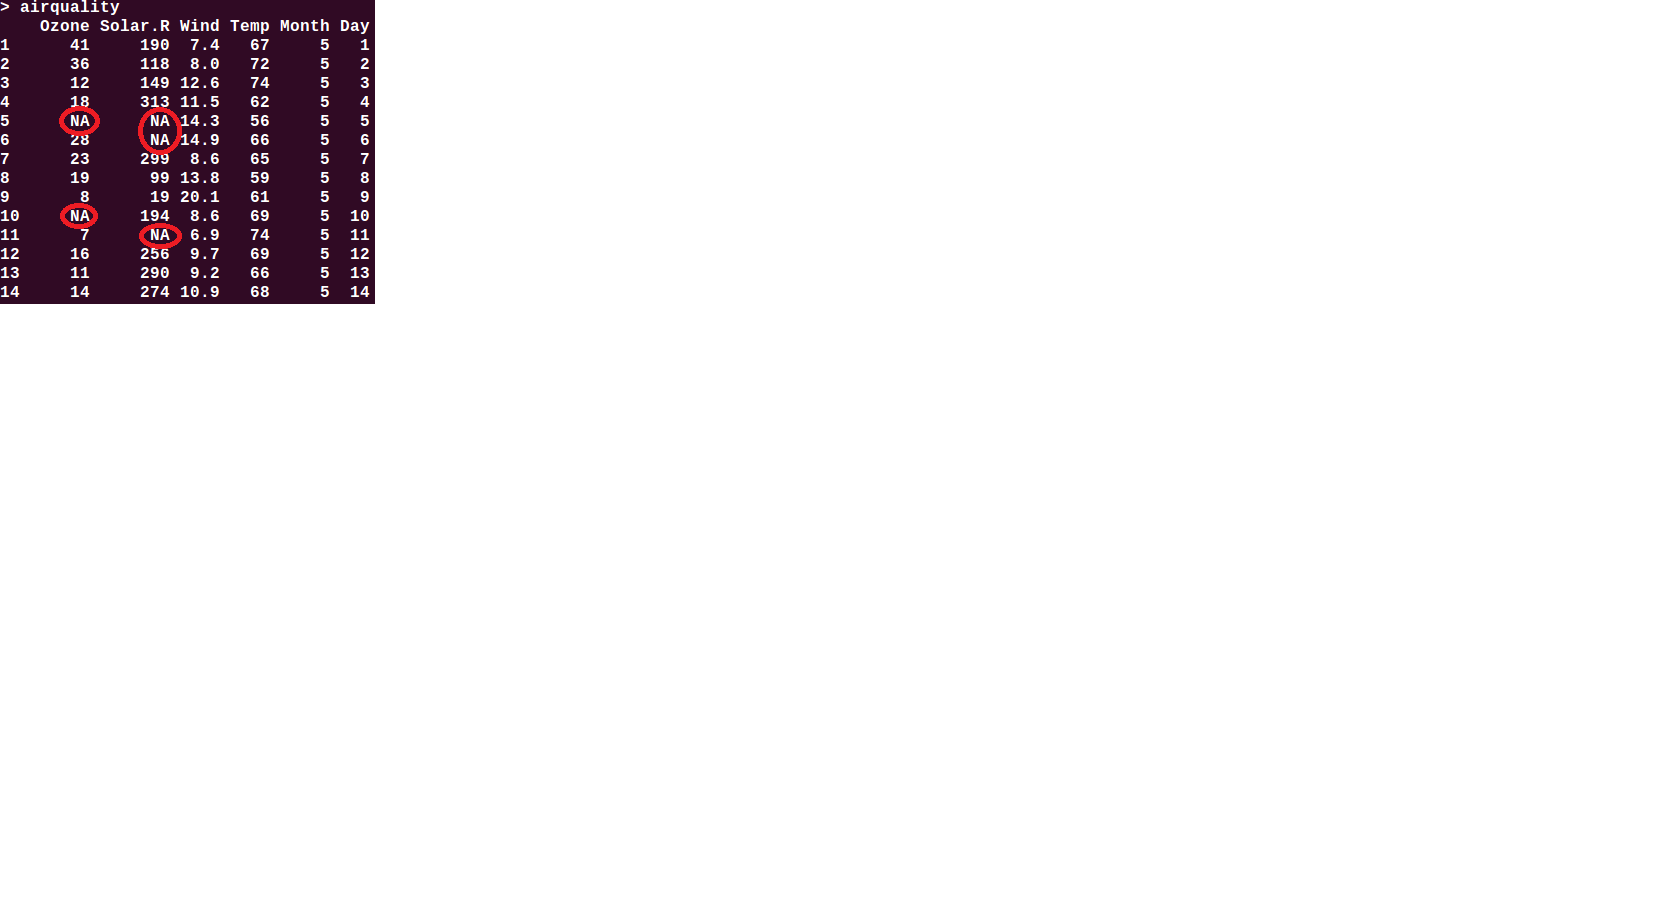
\includegraphics[width=25cm]{images/image_missingvalues.png}
\end{frame}

\begin{frame}
  \begin{enumerate}
      \item<1- | alert@1> 
  \end{enumerate}

  
\end{frame}

\section*{Sommaire}
	\begin{frame}
		  \tableofcontents[]
	\end{frame}      

\section[A simple case]{A simple case : Clinical trial on different antidepressant}
\subsection{case description}
\begin{frame}
	\begin{itemize}
		\item<1->6 centre clinical trial, comparing 3 treatments of depression
		\item<2->367 subjects randomised to one of 3 treatments
		\item<3->subjects rated on HAMD score (0 to 50)  on 5 weekly visits
		\item<4-> Subjects drop out from week 2 onwards (246 complete cases)
	\end{itemize}
	Study objectives : compare efficiency of the 3 treatments over time. metric : HAMD
\end{frame}

\begin{frame}
  \begin{tikzpicture}[remember picture,overlay]
   \node[at=(current page.center)] {
     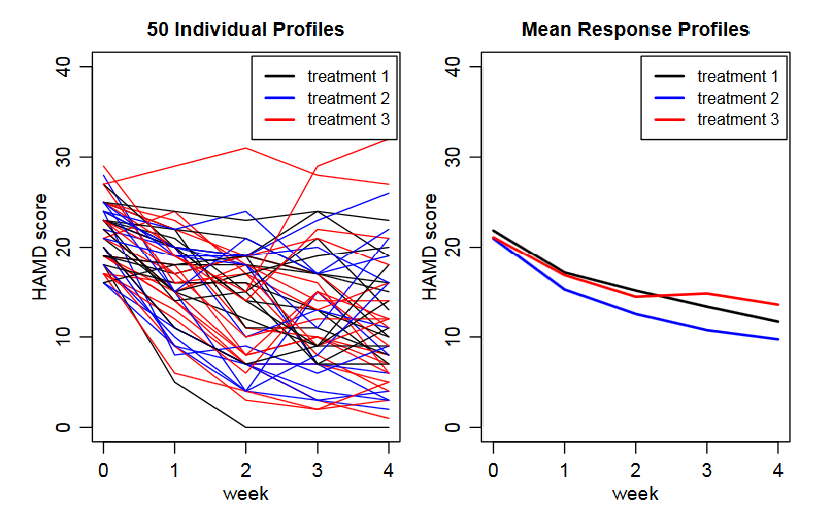
\includegraphics[width=\paperwidth]{images/HAMD_response_profile.png}
     };
  \end{tikzpicture}
\end{frame}

\begin{frame}
  \begin{tikzpicture}[remember picture,overlay]
   \node[at=(current page.center)] {
     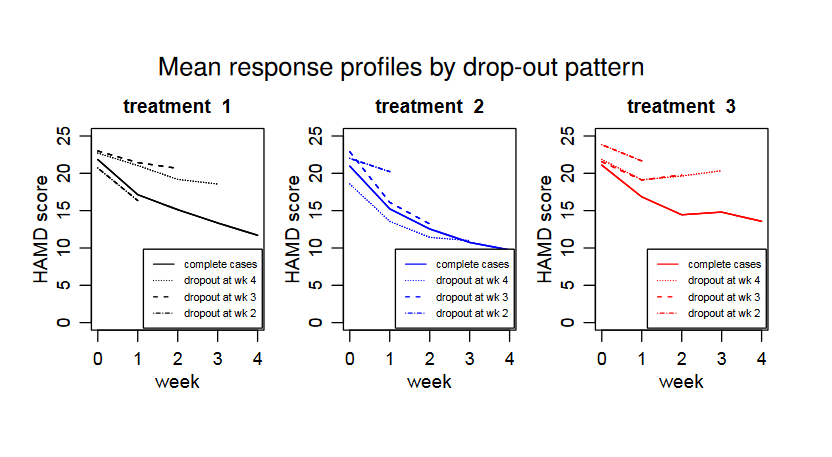
\includegraphics[width=\paperwidth]{images/HAMD_all_response_by_dropout_pattern.png}
     };
  \end{tikzpicture}
\end{frame}


\subsection{What not to do}
\begin{frame}
	\begin{itemize}
	    \item<1->Don't drop uncomplete cases (listwise deletion)
	    \item<2->Don't do Last obeservation carried forward
        \end{itemize}
        \begin{quote}
		Don't mess with missing data \it{Thomas L.}
	\end{quote}
\end{frame}

\begin{frame}
\Huge How would you proceed ?	
\end{frame}

\begin{frame}
	\begin{itemize}
	\item<1->
	\end{itemize}
\end{frame}

\section{references}
\begin{frame}
	\begin{itemize}
		\item<1->Constructing Models to Deal With Missing Data | SciPy 2016 | Deborah Hanus, https://www.youtube.com/watch?v=cHzahWjaA7o
	\end{itemize}
\end{frame}


\end{document}

% some references :
% - Constructing Models to Deal With Missing Data | SciPy 2016 | Deborah Hanus, https://www.youtube.com/watch?v=cHzahWjaA7o
% - http://www.bias-project.org.uk/papers/NonTechnicalMissingTalkSlides.pdf
